\fancyhead[LO]{{\scriptsize {\FA }我们最幸福 {\FA } 17 睁大眼睛闭上嘴}}%奇數頁眉的左邊
\fancyhead[RO]{\thepage}
\fancyhead[LE]{\thepage}
\fancyhead[RE]{{\scriptsize {\FA }我们最幸福 {\FA } 17 睁大眼睛闭上嘴}}%偶數頁眉的右邊
\fancyfoot[LE,RO]{}
\fancyfoot[LO,CE]{}
\fancyfoot[CO,RE]{}
\chapter*{17 {\FA } 睁大眼睛闭上嘴}
\addcontentsline{toc}{chapter}{\hspace{5mm}17 {\FA } 睁大眼睛闭上嘴}
\begin{figure}[!htbp]
\centering
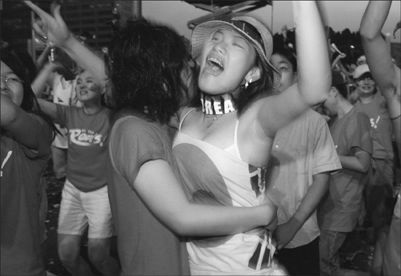
\includegraphics[width=6cm]{./Chapters/Images/17.jpg}
\caption*{2002年首尔庆祝足球世界杯}
\end{figure}


当得知玉熙在农浦,宋女士一点儿也不奇怪。她早就知道女儿会被关进监狱,只是时间早晚的问题。自从玉熙3年前从丈夫那离家出走,她再也没有听说过她的消息。但是宋女士猜想她应该在中国,和那些妓女和叛国者在一起。如果她背叛了祖国,那么蹲监狱是她罪有应得。但是,女儿就是女儿。宋女士不可能眼睁睁的看着自己第一个孩子在清津最臭名昭著的拘留中心里撒手不管。\\

经过多年在死亡在线的挣扎,宋女士吞下自己一个又一个的禁忌。现在她已经精明于人情世故。她早就知道了有钱能使鬼推磨。只要不是因为辱骂金正日而被抓,只要有钱,死刑犯都可以买出来。所以,她跑去黑市,以每包50元的价格,买了10包烟。然后她四处打听,最后找到负责农浦监狱的国家安全局官员。就这样自己那倔强的女儿,一眨眼的功夫就花费了宋女士一整个星期的收入。\\

几天后,玉熙出现在母亲家的前门,旋即昏倒在母亲怀里。\\

当见到她时,宋女士尖叫了一声。此时已经是10月,天已经很冷了,但是玉熙几乎赤裸着身子,光着脚。她的鞋被农浦的警卫切成一块块的,他们以为她会把钱藏在鞋底里。她把自己衬衣的袖子剪下来,以作卫生巾。她的内裤送走了。身上的衣服也破破烂烂。头发里爬满虱子。但是在给她洗澡的时候,宋女士发现玉熙比离开的时候健康的多。即使在监狱里,每顿只能吃到稀粥和地里捡的生玉米粒,但是玉熙骨骼肌肉强健有力,面色红润。\\

玉熙不停的说啊说。精力像山洪爆发一样喷涌而出,她诉说着在中国的一切──他们早饭、中饭、晚饭都吃白米,那里的市场,那里的时尚。她的话一部分是旅游见闻,另一部分是那些抨击政治的陈词滥调。宋女士和两个女儿围着她,听着。\\

“南韩的生活是这样的?”他们问道。\\

玉熙也没有第一手的信息,但是在中国的时候,她看了很多南韩的电视节目。\\

“南韩现在是个富裕的国家。即使是中国人也不敢想象南韩有多么富裕。”玉熙告诉他们。“我发誓在死前一定要去南韩。”\\

当玉熙发誓的时候,妹妹们盘腿坐在地板上。一会儿兴奋、一会儿又感到恐怖。二姐嫁给了个铁路上的警卫,是三个姐妹里最刻板的。随着玉熙的讲述,她的眼睛越睁越大。半信半疑,因为玉熙原来总是唬她,她插话道。\\

“但是我们的将军不知辛劳的为我们…”她指了指母亲今天早上掸过灰的父子画像。\\

“你还看不到?你的将军把你都变成白痴了。”玉熙吼道。\\

小妹容熙,离婚后跟妈妈住,对玉熙的话表示赞同,但是她却担心姐姐的口无遮拦;她们的麻烦已经够多得了。虽然在宋女士的家里可以畅所欲言,但是外面可能隔墙有耳。\\

“小心点,让我们都说话小心点,好吗?”她提醒玉熙。\\

在妈妈和妹妹们对她的故事感到厌烦了的时候,玉熙开始了同其它人的诉说。邻里的大婶们虽然一个个舌头打结,但是好奇心还在。她们一天下午来访,欢迎玉熙的回来,然后聚在她身边听着。\\

“睁开眼睛看看吧。你就能看到我们整个国家就是个监狱。我们就是个可怜虫。你根本不知道外面的世界真正是怎个样子。”\\

无论何时,当金正日的画面出现在电视上的时候,玉熙就会暴怒。“撒谎!骗子!小偷!”她都会朝着电视叫骂。\\

宋女士最后发了脾气。玉熙的大嘴巴会陷整个家庭于危险之中──这是叛国。如果不是自己的女儿说些那样的话,宋女士早就履行人民班的义务而上报了。尽管发生了这么多,宋女士仍然是共产主义的追随者。\\

“闭嘴。你这个国家的叛徒。”宋女士吵玉熙吼道。\\

玉熙一下子懵了──她母亲很少提高她的声音──但是她是不会住嘴的。她马上反唇相讥。\\

“为什么你要把我生在这个可怕的国家?”玉熙喊道。“你更爱谁?金日成还是我?”\\

母亲和女儿之间的争吵就一直没有停。在母亲家修养了40天后,玉熙完全从在监狱里所受的折磨中恢复了过来。她告诉母亲和妹妹们,她已经从先前的错误中吸取了教训,现在她要再试试,去中国赚钱。不同的是,这次她不会再被抓住了。宋女士很不情愿的又给了玉熙一些钱。她非常担心,但与此同时,当女儿离开时又松了口气。\\

一晃8个月过去了,玉熙没有稍一句话回家。之后,在6月里,一个女人到了宋女士家门口,声称有女儿的消息。宋女士振作了下精神。玉熙一定是又被关进监狱了。她又要不得不想办法把她弄出来。但是,这次却不是,这个女人说玉熙在靠近中国边境的地方工作,近况很好。她想把借妈妈的钱还给她,还买了些衣服和礼物给家里人,但是如果回清津的话,她害怕会被逮捕。所以宋女士能不能去她那里走一趟。\\

宋女士犹豫了。她不认识这个女人。自从1995年出事故的那次,给家里带来巨大痛苦的行程之后,她再也没有出过远门。她其实不需要钱;她的饼干生意还过得去。现在松片市场提供摊位给商贩们,整个市场也安装了顶棚。她付租金,还领了执照。现在她觉得自己像个正正经经的女商人。她也再婚了──是形式上的。其实更像是一种安排,寡居、年长的女人家里需要一个男人相互照应,但是那人很善良,经济状况也比较好。宋女士现在的日子过的比以前舒适多了。她没有理由要冒险去中国边境,但是她又有点心疼上次弄玉熙出来时花的那500块钱。这个陌生女人向宋女士许诺她不用坐火车──玉熙已经安排好了一部私人汽车。这打动了宋女士,之后她就同意了。\\

在2002年6月一个闷热多雨的一天,宋女士出发前往茂山。她只随身带了个小行李包。她打算只在那里过一夜,第二天早上就回来。但是当他们到了那里的时候,根本没有玉熙的影子。一开头,宋女士只是被告知女儿在边境地区工作。但是这个妇女没有说是边境的哪一边,现在事实很清楚了:玉熙在中国。\\

“你要去中国拿衣服和钱。你的女儿在那边等着你。”这个女人告诉她。然后她介绍了个说是自己丈夫的男人给她。“别担心,他会带你去的。”\\

宋女士已经走了这么远。难道她现在要回头吗?于是,他们乘了另外一部车驶向通往另一个边境城市会宁的路。之后他们在那等着天黑。\\

当他们到达河边的时候,已经是晚上10点,天还下着雨。河水暴涨,激流拍打着河岸,溅了他们一身泥水。宋女士几乎分不清哪里是河岸,哪里是河水。两个穿着北朝鲜边境警卫制服的男人和他们汇合。一个人像拎孩子一样把宋女士背在背上,另一个则握住第一个人的手臂,在过河的时候帮助他们保持平衡。他们趔趄了好几次,几乎失足。宋女士以为她肯定会落水并被激流冲走。像她那一代大多数的北朝鲜人一样,她不会游泳。但是正当宋女士挣扎着冒出水面,并能喊出心中希望的──带我回去,带我回去──之前,他们爬上了对岸。一个向导给了这两个边境警卫一些钱,然后他们就掉头回了北朝鲜,消失在视线之中。宋女士和另外一个向导抹黑进入了中国,连夜翻越了一座小山,在天蒙蒙亮的时候,来到了一个小村庄。\\

之后他们坐进了一部出租车,这是宋女士从来没坐过的东西。汽车、卡车、摩托车,然后是马车沿着一条窄窄的街道,到了一个市场。市场里喇叭声此起彼伏,此时早上8点了,商店都开门了。橱窗前的卷帘门被拉起,发出一阵刺耳的金属刮擦声。店主们纷纷打开音乐,声音从放在门口的扬声器传送出去。震耳欲聋,可怕的音乐,宋女士想。她想用手指把耳朵堵住。如果这就是资本主义,她不喜欢。太嘈杂了。玉熙怎么能在这么可怕的地方待下去?\\

宋女士的向导停下脚步,买了鸡蛋、香肠和猪脚作为早餐。然后他们出了镇子,沿着一条土路来到了一簇房子形成的一个小村庄。他们进入了其中的一栋房子。向导把宋女士介绍给了这栋房子的男主人和他十几岁的女儿。他们都是朝鲜族的中国公民,说和宋女士一样口音的朝鲜语。他们带宋女士四处看了看。这栋房子没什么特别的──红砖墙,瓦屋顶,自制的木栅栏在房子前面围了个院子──但是屋子里塞满了各种电器:一个立体声音响、一个饮水机、一台彩电、一个冰箱。那个男人不断的打开冰箱,拿出很多吃的、喝的。啤酒、水果、泡菜。然后向导把买的吃的也摆在一起的时候,满满一桌子,比宋女士在婚礼上的酒席看到的还要丰盛。她可能想要的所有东西都在这儿了,所有东西,除了玉熙。\\

“我女儿在哪里?”宋女士问道。\\

那个男人看着她,嘟囔些她听不懂的东西。宋女士又问了一次,这次更急切了。\\

“她出去找工作了。”他答道。宋女士不知道该不该相信他。她的房东很好,简直太好了:宋女士认为他们正在隐瞒什么东西,但是她实在太累了不想去深究。她迷迷糊糊的睡着了。当她起来后,仍然没看到玉熙,突然她脑海里闪现出一个可怕的设想:她被绑架了。\\

宋女士不知道她现在是不是该逃跑。她又能跑到哪里去呢?她连自己身处何方都闹不清楚。最初的向导走了。因为自己的怀疑,她是不是该采取些反抗措施?她女儿怎么样了?这对夫妇不停的宽慰她,说玉熙有事情耽搁了,马上就会回来。第二天,玉熙终于打电话过来了。电话里声音很嘈杂,仿佛她是从很远的地方打来。她试图宽慰母亲她一切都很好,她很快就能见到她了,现在她应该好好休息。\\

“你到底在哪里啊?”宋女士疑惑的问道。\\

“在韩国(Hanguk)。”玉熙回答。\\

宋女士从来没听说过这个地方。\\

“那是那里啊?靠近沈阳吗?”宋女士问道,提了一个中国东北地区最大的城市,大概离她现在的住地有500公里。\\

“还要远。我明天打电话给你解释。”\\

北朝鲜人称呼他们的国家为朝鲜(Chosun)而称呼他们分离的邻居南朝鲜(Nam Chosun),字面意思就是South Korea(南朝鲜)。而南韩人则用完全不同的称呼称他们自己的国家。他们称为韩国(Hanguk)。\\

在下一次电话中,玉熙说明了她实际是在南韩。宋女士简直不敢相信。她是如此愤怒,全身气的发抖。她担心自己会犯心脏病。在玉熙做的所有坏事中,从小时候的恶作剧,到后来她的一张臭嘴,再到被关进监狱,这次是最出格的一次。她竟跨境投敌了。她雇佣这些人诱骗母亲叛逃。宋女士一生里从未如此愤怒过。\\

“你个叛徒!你不是我女儿。”她对着电话咆哮着,之后重重的摔掉听筒。\\

随后的几天里,玉熙反复的打电话过来。宋女士拒绝接电话。最后,她心软了。\\

玉熙在电话里抽泣着。\\

“妈妈,我爱你。我想你能来和我一起住在这里。”玉熙告诉了她一点自己现在的生活。她找了份工作。南韩政府也给了一笔钱作为安家费。\\

“如果在首尔的生活这么好,干什么还哭?”宋女士问道。\\

宋女士认为南韩就是美帝国主义的傀儡,一定是用钱买通了她女儿。一旦从玉熙身上榨取到所需的信息,他们就会折磨她、杀害她。这就是宋女士曾经听说的南韩如何对待北朝鲜叛逃人员的传言。她没有理由不去相信这些。\\

“不是这样的,妈妈。”玉熙反驳道。“我哭是因为我想你,我想你来这里。”\\

宋女士不想听。她告诉玉熙一旦她休息好,她就要回到北朝鲜。她要休息几天,攒点力气。\\

在此期间,她就房前屋后的转悠转悠,发发呆,吃吃东西,看看电视。房子里有个很大的白色卫星天线,可以接受南韩的电视节目。在这里,南韩的肥皂剧很受欢迎,宋女士也很快就喜欢上一部叫水晶鞋的电视剧,说的是两个父母双亡的姐妹,从小分离的故事。当没有电视节目的时候,她就草草浏览些其它的频道,找找足球比赛。\\

2002年足球世界杯由南韩和日本联合举办。自从1988年南韩举办奥运会以来,还没有如此多来自首尔的镜头。宋女士对足球不感兴趣,但是她想通过那些比赛的背景镜头,看一看南韩。她不可能注意不到那些汽车、高楼大厦、商场。在电视插播广告的间歇,都是行动电话的广告还有些东西宋女士是闻所未闻。\\

当南韩击败波兰、踢平美国,之后,又接连击败葡萄牙,意大利,和西班牙杀入半决赛──有史以来第一支亚洲球队进入到四强──数以百万的人们涌向街头疯狂庆祝。人们都穿着红色的T恤,戴着会发红光的小犄角──这种球迷俱乐部的装束,号称红魔。那里,他们都是朝鲜人,就像她一样,说同一种语言,但是他们看上去是如此俊美、如此欢快而且如此自由。\\

要相信电视上看到的一切,对于宋女士来说很难。在北朝鲜待了一辈子,她很清楚(更不用提这些年里和一个记者25年的婚姻)所见未必是真实,一切都是可以操纵的。劳动党的讲座也提醒她外国的电视节目是专门制作的用于颠覆金日成和金正日的教导\footnote{“在美国中情局操纵之下,南朝鲜傀儡政权用心险恶的用一些专门制作的材料来美化帝国主义。”一个讲座里曾这样说。}。她怀疑这些的正确性。她那慷慨的房东也是玉熙雇来的,帮自己洗脑后去南韩。\\

但是也不可能所有的都是假像。她不可能否认自己在中国看见的──充足的食物、汽车、家电。\\

她的房东有个自动的电饭煲、带有感应器、在煮好饭之后就会自动关掉。他们大多数的家电都让她感到好奇,单单是这个电饭煲就是个无尽的神奇之源。很久以前,她也曾有个煮饭的电饭锅,但是和这个太不一样了。后来还被警察没收了,因为你不允许用电煮饭。\\

每天早上,她都可以听见电饭锅哔的一声,说明饭煮好了,宋女士惊奇于现在的科技。这是真的,她现在认为,北朝鲜是几年,甚至几十年的落后于中国。但是谁又知道落后南韩多少年呢?她怀疑她那可怜的前夫可能早就知道她现在在中国看到的一切。虽然到了之后,就没离开过那栋房子,但是仅仅是看看厨房,换换电视频道,对于她来说已经是个巨大的奇遇了。她要将这一切同丈夫分享。她总是想到长博,特别是吃饭的时候。他是个多么爱吃的人啊!他一定会喜欢这个香肠的。想到这里,她泪水涟涟。然后她又想到了自己的儿子。她的记忆里满是负罪和愧疚,她甚至不曾好好和他推心置腹的谈过。他曾经是那么的强壮,那么的英俊──多么不幸啊,才25岁就去世了。他失去了多么美好的生活啊。他们都失去了多少啊,自己、女儿们、被囚禁在北朝鲜,辛劳工作到死,为了什么呢?我们按党的教导做。我们誓死为将军。我们无所羡慕。我们走自己的路。她曾经相信这些,她已经虚度年华。或者并不是。一切真的过去了吗?她才57岁,身体还硬朗。\\

当晨曦淡淡的光透入房间时,这些想法不停的在脑子里回荡。正在苦思冥想之时,她听见厨房的电饭煲哔的一声。她起了床,一天又开始了。这就是她的起床信号。她准备好走了。\\
